\def\year{2015}
%File: formatting-instruction.tex
\documentclass[letterpaper]{article}
\usepackage{aaai}
\usepackage{times}
\usepackage{helvet}
\usepackage{courier}
\usepackage{graphicx}

\frenchspacing
\setlength{\pdfpagewidth}{8.5in}
\setlength{\pdfpageheight}{11in}
\pdfinfo{
/Title (Genkii - The Effects of Varying Sequential Rewards for User's Motivation to Complete a Set of Crowdfunded Tasks.)
/Author (Helmut Prendinger, Ruben Geraldes, Daniela Fontes, Daniel Morais, Rui Prada)
/Keywords (Crowdsourcing)}
\setcounter{secnumdepth}{2}  
\setlength\titlebox{8cm}
 \begin{document}
 
% The file aaai.sty is the style file for AAAI Press 
% proceedings, working notes, and technical reports.
%
\title{Genkii - The Effects of Varying Sequential Rewards for User's Motivation to Complete a Set of Crowdfunded Tasks}
\author{Ruben Geraldes \\
rubengeraldes@gmail.com \\
Instituto Superior T\'{e}cnico, \\ Universidade de Lisboa,\\
	Av. Prof. Cavaco Silva, \\ Taguspark Porto Salvo, Portugal\\ 
	\And Daniela Fontes\\
	daniela.fontes@ist.utl.pt \\
	Instituto Superior T\'{e}cnico, \\ Universidade de Lisboa,\\
	Av. Prof. Cavaco Silva, \\ Taguspark Porto Salvo, Portugal\\
	\AND Helmut Prendinger \\
	helmut@nii.ac.jp\\
	National Institute of Informatics,\\
	2-1-2 Hitotsubashi, Chiyoda-ku, \\ Tokyo, 101-8430, Japan \\ 
	\And Rui Prada\\
	rui.prada@tecnico.ulisboa.pt\\
	INESC-ID ,\\
	Av. Prof. Cavaco Silva, \\ Taguspark Porto Salvo, Portugal\\		
}



\maketitle

% If the title and author information does not fit in the area allocated,
% place \setlength\titlebox{height}
% after the \documentstyle line
% where {height} is something like 2.5in

\begin{abstract}

Genkii is a GPS enabled mood reporting application. In this work we plan and execute a crowdsourced study using Yahoo Japan. Given a reward budget per user, we study the influence of offering a fixed reward in comparison to an increasing reward scheme. Even though the two methods perform very similarly, using an increasing reward scheme increases user completion of the set of tasks.

\end{abstract}

\section{Introduction}

\subsection{Motivation}



The ubiquity of hand-held devices opened up new opportunities for research. Nowadays it is accessible to perform off-site studies and collect data in real-time and across great geographical spans.

One of the ways to deploy these off-site studies is by using micro-tasks markets. We are specially interested in this type of crowdsourcing.

This new paradigm also gives rise to the search for new methodologies, and best practices, which may help the scientific community improve and stage new experiments, in a way that optimizes its resources.



Genkii was conceived after realizing some problems in attracting users for crowdsourced studies in Japan. The initial hypothesis for this problem in attracting users for social studies had to do with privacy issues.

We want to study the effects of varying inducements to get people to perform a determined task repeatedly.

\subsection{Outline}

\section{Related Work}
\subsection{Crowdsourcing}
\label{subsec:Crowdsourcing}

In order to set up a crowdsourcing campaign we use the framework suggested in \cite{Henze2013}.

\begin{enumerate}
		
\item Clearly identify the research goals; \item Select a study method; \item Devise an incentive mechanism;  \item Choose the target platform(s); \item Design and develop the mobile app; \item Prepare data collection; \item Implement a scheme to obtain informed consent from users; \item Distribute and promote the app; \item Continuously monitor data collection for a designated time period; \item Filter and analyze data to answer the research question
\end{enumerate} 
\cite{Henze2013}.


\subsection{Rewards and Motivation}



\begin{quote}
When explicit incentives seek to change behavior in areas like education, contributions to public goods, and forming habits, a potential conflict arises between
the direct extrinsic effect of the incentives and how these incentives can crowd
out intrinsic motivations in the run short and the long run.
\end{quote}
\cite{Gneezy2011}




The use of rewards to induce a desired behavior has been thoroughly studied. 
There has been a clear separation between intrinsic rewards and extrinsic rewards, and research points out that a high focus on incentives can ultimately lead to the alienation of creative thinkers. 
According to \cite{Gneezy2011}, there are instances where monetary rewards (extrinsic rewards), work well. Mechanical based, self-contained and well-specified tasks seem to be the primary candidates for the usage of extrinsic rewards to motivate, induce or boost the agent's performance\cite{Ariely2009}.

Crowdsourcing is often associated with Gamification, the use of game-design elements to achieve a more compelling user-experience driven by fun.


However there is criticism when using incentives in areas like education and forming habits, because they can hinder natural intrinsic motivation, and the dependence on rewards may lead to reward inflation, and lower the effort the agent is willing to put towards the task \cite{Irlenbusch2005}. 





\subsection{Crowdsourcing Platforms}


\subsubsection{Amazon's Mechanical Turk}

Amazon's Mechanical Turk is a platform which serves as an interface for the deployment of crowdsourced tasks that are considered easier for humans than machines. 

It creates a labor market in which individuals or corporations can list tasks (also known as HITs or “human intelligence tasks”), and a specified compensation. The workers can then elect to complete a determined task, against a deadline, and be compensated upon timely completion. The compensation for the worker is either being paid a determined amount, or a free volunteered work \cite{Mason2010}. 
This model has been referred to in the literature as a micro-tasks market\cite{Kittur2008}.

In \cite{Mason2010} it is shown and discussed the potential use of Amazon's Mechanical Turk for laboratory experiments for a low fee (between 0.01\$ and 0.10\$).
The main advantages cited for the merit of these studies are the convenience of the platform in reaching many users in a relatively short notice and it is mentioned that the average cost per user is very low, in the order of cents per task.
Also it has been shown \cite{Kittur2008} that, provided that the type of task is well-specified, easily measurable, and do not put a lot of emphasis on creativity,  the quality of work performed on Amazon's Mechanical Turk is as good, and maybe even better than, work performed by experts paid under traditional contracting arrangements.

Further experiment design recommendations offered in \cite{Kittur2008} including the concern in devising the tasks such that it discourages random or malicious completion, by making a good performance require the same or less effort than a tampered one.


\subsubsection{Yahoo Crowdsourcing Japan}

Yahoo Crowdsourcing Japan works in a similar way as the Amazon's Mechanical Turk. 


\section{Genkii}


Genkii is an application that enables gps localized satisfaction reports. Users report their ''Genkiiness'', by performing three different gestures:

\begin{itemize}
	\item Circle meaning that the person feels happy/genkii;
	\item Triangle which represents an ''OK'' state;
	\item Cross which denotes sadness.
\end{itemize}





\subsection{Implementation}
\label{subsec:implementation}



\subsection{Crowdsourcing Campaign}



Following the methodology suggested by \cite{Choi2014}, we want to perform a study where one group will be considered our baseline by receiving a fixed reward for each task over time.
Besides our control group, we devise a second incentive scheme, that using the same amount of points, poses as a progressive reward system. We can compare both reward schemes on \ref{tab:rewards}.

Our goal is to study this and compare these two incentive schemes, specially by studying user enrollment rates and user drop rates.

\begin{table}[!h]
	\caption{ Scheme of rewards used for the crowdsourcing campaign. Using the same amount of reward points, for our first group these rewards are the same for every task over time. On the second group, we devised an increasing reward mechanism. }
	\begin{center}
\begin{tabular}{|c|c|c|c|c|}
	\hline  Reward & Task 1  & Task 2  & Task 3  & Task 4 \\ 
	\hline  Stable Rewards & 20 & 20 & 20 & 20  \\ 
	\hline Increasing Rewards & 5 & 10 & 15 & 30  \\ 
	\hline 
\end{tabular} 

\begin{tabular}{|c|c|c|c|c|c|c|c|c|c|c|}
	\hline   Task 5 & Task 6 & Task 7 & Task 8 & Task 9 & Task 10 \\ 
	\hline   20 & 20 & 20 & 20 & 20 & 20 \\ 
	\hline   35 & 40 & 50 & 60 & 60 & 60 \\ 
	\hline 
\end{tabular} 
\end{center}
\label{tab:rewards}
\end{table}

As stated in Section \ref{subsec:Crowdsourcing}, we followed the framework proposed in \cite{Henze2013}.
\begin{enumerate}
	\item Our main research goal is to compare two different reward schemes using the same budget per user (fixed rewards versus increasing rewards), on a set of sequential tasks;
	\item We are going to compare user on-boarding and drop rates in order to understand how do the two rewards perform;
	\item By using Yahoo Crowdsourcing we award ''T-Points'', a popular loyalty points card;
	\item The target platform of the Genkii App is Android;
	\item We discuss the design of the application in detail on Section \ref{subsec:implementation} . We focused on creating a user interface using gestures, which makes the interaction with the application uncommon;
	\item Before launching the campaign featured in this study we performed several pilot tests, which enabled us to understand the Yahoo Crowdsourcing platform; 
	\item After the installation we present a tutorial where we explain the type of data collected, and the terms in which the data will be used;
	\item The Yahoo Crowdsourcing is an interesting solution to distribute our application, since it handles the promotion;
	\item During the campaign we monitor for the server uptime, ensuring the data is being properly retrieved;
	\item The last point has to to with filtering and answering the research question. In the following section we present and discuss the results obtained.
\end{enumerate}


The first campaign ran from 19/06/2015 to 26/06/2015. The second campaign featuring increasing rewards ran from 08/07/2015 to 15/07/2015.

%\subsection{Individual versus Group Analysis}
%
%One of the main concerns for the analysis of this experiment is whether to consider the aggregated group behavior or the individual behavior.
%
%After all our objective is to compare two reward schemes, and test our hypothesis. 
%
%** If we consider the group of users a system, then the aggregated behavior can be considered a legitimate approach, as we are interested on the overall behaviour of the system, when designing a large scale study. 
%
%An analogy is the way we study and understand temperature in Physics. Temperature is defined as a measure of the average kinetic energy of the particles in a system. We can define, derive, and predict an enormous range of behaviours, by measuring the temperature of the system. However the behaviour of an individual particle in the system, and its kinectic energy, is complex and difficult to associate with the behaviour of the group of particles.
%
%is a measure of the average kinetic energy of the particles in a system
%
%*theory of ergodicity

\subsection{Expectations and Hypotheses}

Intuitively we expect the fixed reward scheme to have a greater on-boarding, with more players joining in enticed by a considerable reward. On the other hand, we expect less players joining the increasing reward version, but those who join will be motivated to get bigger and bigger rewards.

This experiment is going to be deployed in the Japanese population via Yahoo Crowdsourcing. Genkii, as a location enabled mood reporting application, allows the capture of interesting informations about its users. Even though there may be validity issues regarding the accuracy of Genkii to relay truthful reports, the system is designed in a way that the effort to report a false mood is exactly the same as for reporting the actual mood evaluated by the user, according to the best practices referred in \cite{Kittur2008}.

 We hope we will be able to capture some insights about the people who use this service.
 
 We also expect to collect a set of best practices, and lessons learned that can be applied to future crowdsourced studies, in particular those using Yahoo Japan.  

%suggestion sentiment annalysis with Genkii
\section{Results}

The first campaign featuring a fixed reward scheme counted with 436 genkii reports.
115 users installed the Genkii application, and 79 users provided at least one report.

The main goal of this study is to compare the effect of rewards on the user's reporting behaviour.
At first glance in order to understand the data collected it's important to study the overall frequency of the user reports. In the Figure \ref{fig:freqreports1} we can observe that in fact there seems to be considerable on-boarding effect with 39 users making 1 report. But we also have a group of 15 users that made more than the strictly required (10 reports).

\begin{figure}[htb]
	\begin{center}
		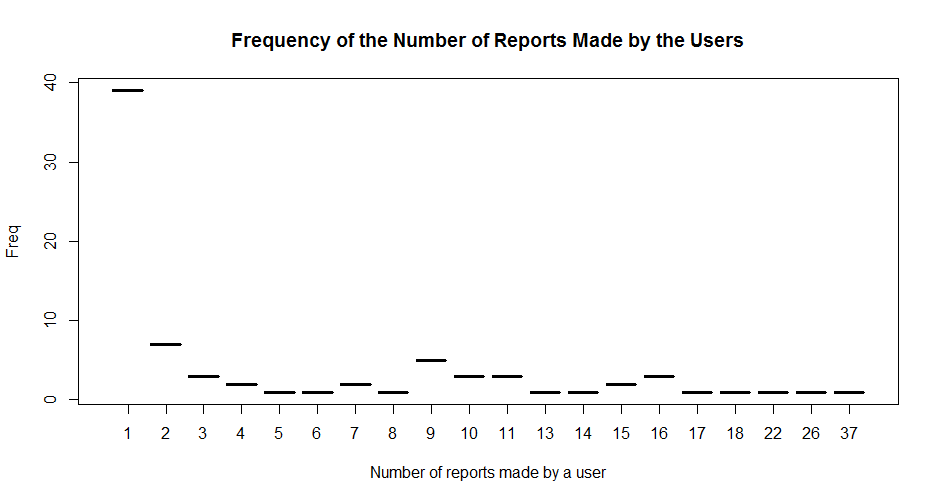
\includegraphics[width=1\linewidth]{images/FReports}
		\caption{Frequency of reports made by users during the fixed reward campaign. As expected, the number of users that made only a single Genkii report (39) stands out. On average each user makes 5.5 reports with a standard deviation of 6.9 reports, the median is 2 reports.\label{fig:freqreports1}}
	\end{center}
\end{figure}

As we can observe in Figure \ref{fig:freqreportsperday1} the campaign quickly took off. During the last three days we verified a drop in the number of reports being made. Our hypothesis for this has to do with the architecture of the Yahoo crowdsourcing and a limit of times the each task could be unlocked, as we were primarily interested on studying the sequential behavior. Also users understood that given the time constraint between reports (4 hours), it was became more difficult to finish the set of 10 tasks.

\begin{figure}[htb]
	\begin{center}
		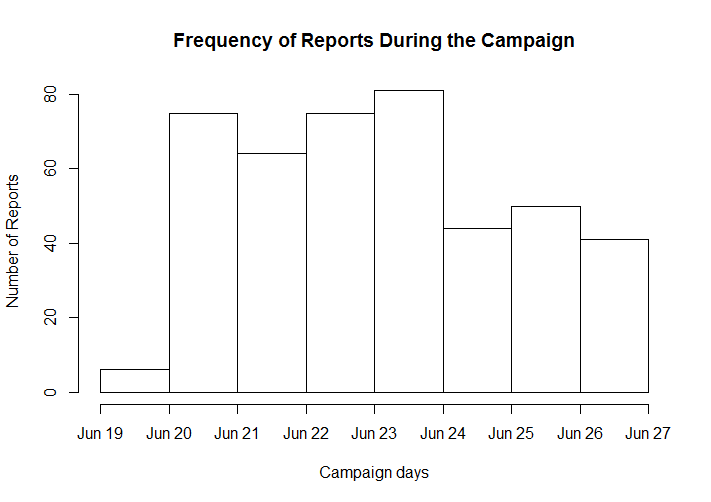
\includegraphics[width=1\linewidth]{images/RPerDay}
		\caption{Number of Reports made on each day of the fixed reward campaign campaign.\label{fig:freqreportsperday1}}
	\end{center}
\end{figure}

\begin{figure}[htb]
	\begin{center}
		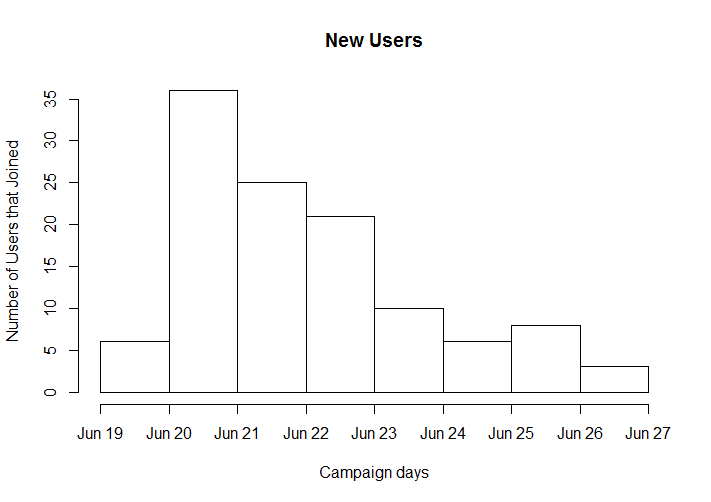
\includegraphics[width=1\linewidth]{images/NewUsers}
		\caption{User acquisition throughout the fixed reward campaign.\label{fig:newusers1}}
	\end{center}
\end{figure}


The increasing reward campaign run from 08/07/2015 to 15/07/2015.
123 users installed the Genkii app during the campaign, with 94 users providing at least one report. We captured 623 Genkii reports during this campaign.

%This makes the second campaign 


\subsection{Reward Schemes}

In order to compare the two incentive schemes devised we use the user drop rate as a metric for how well the users stick with our 10 task program.

We verified that 9 users completed the 10 rewarded tasks during the fixed campaign reward. It is important to refer that in order to unlock a reward the reports have to be made with a 4 hour interval. There were 18 users who ended up making 10 or more reports, during the fixed reward campaign.

When using the increasing reward scheme we noted that 16 users finished the 10 rewarded tasks. Taking into account the user participation in the two campaigns, we can conclude that users on the increasing rewards scheme were more likely to finish the tasks (17\%) in comparison with the fixed rewards scheme where only 11.3\% of the users completed the 10 rewarded tasks.
In the increasing rewards campaign 25.5\% of the users did more than 10 reports, in the fixed reward scheme 22.8\% did more than 10 reports.


Overall user participation decreases sharply during the first two quests, on both campaigns.
The most notorious difference between the two campaigns is the drop experiences between the first and second quest. 
The fixed reward scheme has an initial drop rate of 50\%. After the first reward, 35\% of the users did not claim any more rewards on the increasing reward incentive scheme.  
In the increasing reward scheme the users have a smaller drop rate between the first and second quest, with 15\% more users remaining in comparison with the fixed reward scheme.

Besides the transition from the first to second quest, there seems not to be a major difference in the way the two populations decrease throughout the experiment. 
However the increasing incentive scheme has a large drop rate (18.2\%) between the second reward and the third reward, compared with the drop experienced in the fixed reward scheme (7.3\%). 
The mean difference between the two sets is -3.1\% (with a standard deviation of 5\%), the fixed reward scheme having a larger drop rate predominantly. However if we do not consider the drop rate that happens on the second task, there is an average -1.8\% (with a standard deviation of 2.9\%), difference between the increasing rewards and the fixed reward. This points us to the fact that the increasing reward scheme provides a slightly higher incentive to keep users on track.



\begin{figure}[htb]
	\begin{center}
		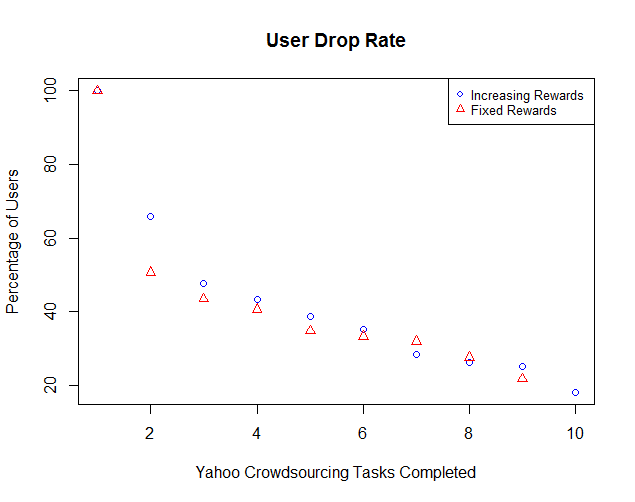
\includegraphics[width=1\linewidth]{images/UserDropRate}
		\caption{Comparision of the user drop rate for the fixed reward scheme and the increasing reward incentive scheme.\label{fig:UserDropRate}}
	\end{center}
\end{figure}

The percentage of rewarded reports during the fixed reward campaign was 64.8\%.
In the increasing reward campaign the proportion of awarded reports is 62.3\%. Although the difference between the two campaigns is 2.5\%, users on the increasing reward campaign appear to be more predisposed to report without receiving a reward.

Considering all the reports obtained using two different reward schemes, we verify that the reward does not seem to have an impact on the overall emotional reports captured. This effect can be observed in Figure \ref{fig:RewardedvsNonRewarded}.
 
\begin{figure}[htb]
	\begin{center}
		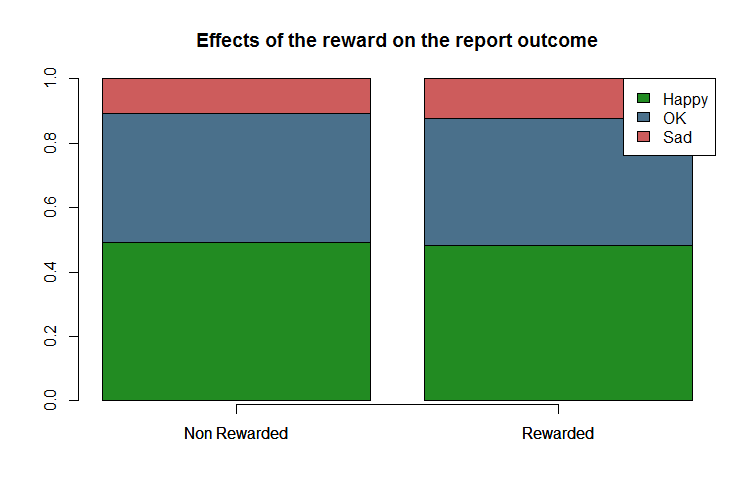
\includegraphics[width=1\linewidth]{images/RewardedvsNonRewarded}
		\caption{The rewards given do not affect the proportion of emotions reported.\label{fig:RewardedvsNonRewarded}}
	\end{center}
\end{figure}

Between reward incentives, the fixed reward scheme also verifies the trend displayed in Figure \ref{fig:RewardedvsNonRewarded}, with very slight differences in the overall emotional reports obtained. On the increasing reward scheme, however we found that these differences in the emotional reports were more accentuated the rewarded reports displaying a higher ''Feeling Sad'' percentage \ref{fig:RewardedsIncreasing}.

\begin{figure}[htb]
	\begin{center}
		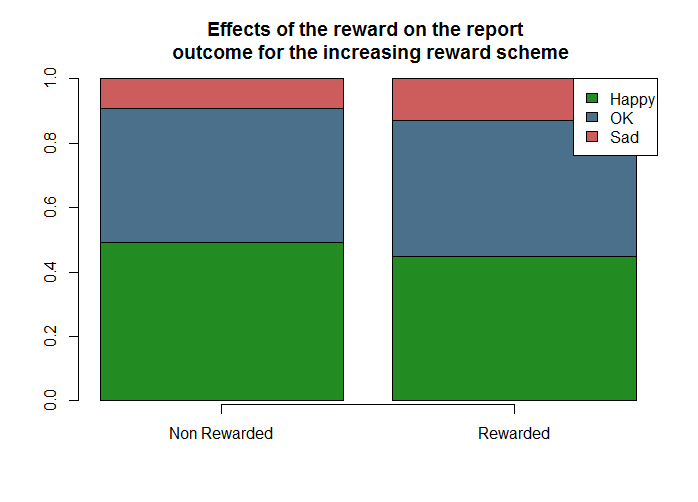
\includegraphics[width=1\linewidth]{images/RewardsIncreasing}
		\caption{Difference between the proportion of  the different emotional states when the report is rewarded or not.\label{fig:RewardedsIncreasing}}
	\end{center}
\end{figure}




\subsection{Genkii Territory}

As location enabled emotional report application, Genkii provides insights on the location of the users, and overall mobility.

To capture mobility information we created the concept of ''Genkii Territory'', which we define as the area that spans between the maximum and minimum latitude and the maximum and minimum longitude reached by a player, adjusted for the earth shape, by assuming a sinusoidal projection. This area is an estimate of overall mobility.
It is important to keep in mind that we limited the ability to report consecutively on the same location.

We calculated the "Genkii Territory" for all players that report at least 6 times during both campaigns. There were 65 users that fit the requirements set.

Given the fact that the distribution of the areas that we obtained (in $km^2$),
has a great variance, the standard deviation is 19105.4$km^2$, the mean being 4698.00, and the median 81.72. We categorize the players, regarding their mobility according to the bins in Figure \ref{fig:territory}.

Most of the Genkii users who report more often seem to travel daily distances associated with commuting. Either those who stay practically on  the same spot (''House Dwellers''), or those who travel long distances seem to be a minority.

\begin{figure}[htb]
	\begin{center}
		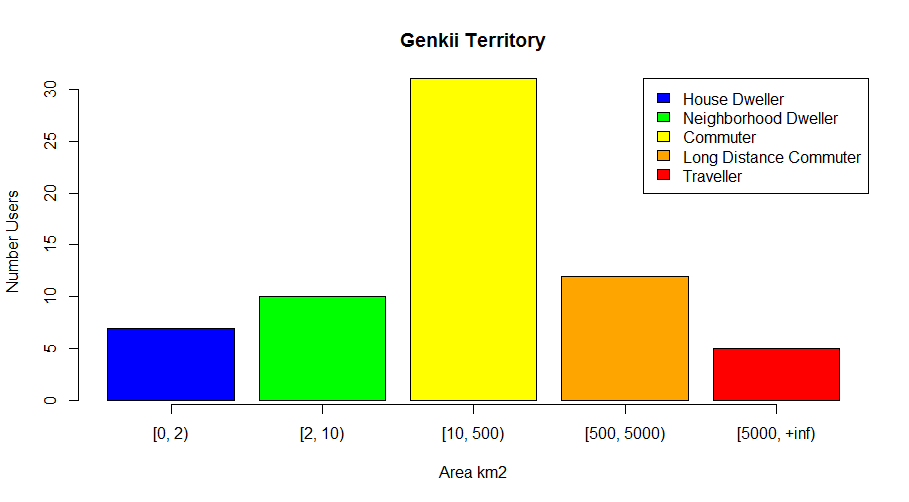
\includegraphics[width=1\linewidth]{images/territory}
		\caption{Genkii territory. Given approximate sizes of cities, we figured 5 category ranges to classify our users with regards to their mobility. Those who have a ''Genkii Territory'' that spans for less than 2$km^2$ are called ''House Dwellers''. If they have a territory no larger than 10$km^2$ they are classified as ''Neighborhood Dwellers''. Most of our users have a territory comprised between 10$km^2$ and 500$km^2$ we figured these values could be common for commuters.
			We also define a '''Long Distance Commuter'' category. And for  users which have a ''Genkii Territory'' larger than 5000$km^2$ we supply a ''Traveller'' label. \label{fig:territory}}
	\end{center}
\end{figure}




\subsection{Genkii Distribution}

In order to capture trends over time we user all the reports collected during both campaigns.
With these results we seek to understand more about the users who signed with Yahoo Crowdsourcing to provide Genkii reports.

The mean proportion of registered emotions is 49\% of ''Happy reports'', 39\% of ''OK'', and 12\% of ''Sad'' Reports.


In the Figure \ref{fig:genkiioverday} capture the hourly distribution of the reports. We can observe that there seems to be a cyclic pattern during the day, with the lowest amount of reports made at 1, 9, and 17. Culturally it is interesting to verify that these are common commuter times. 
\begin{figure}[htb]
	\begin{center}
		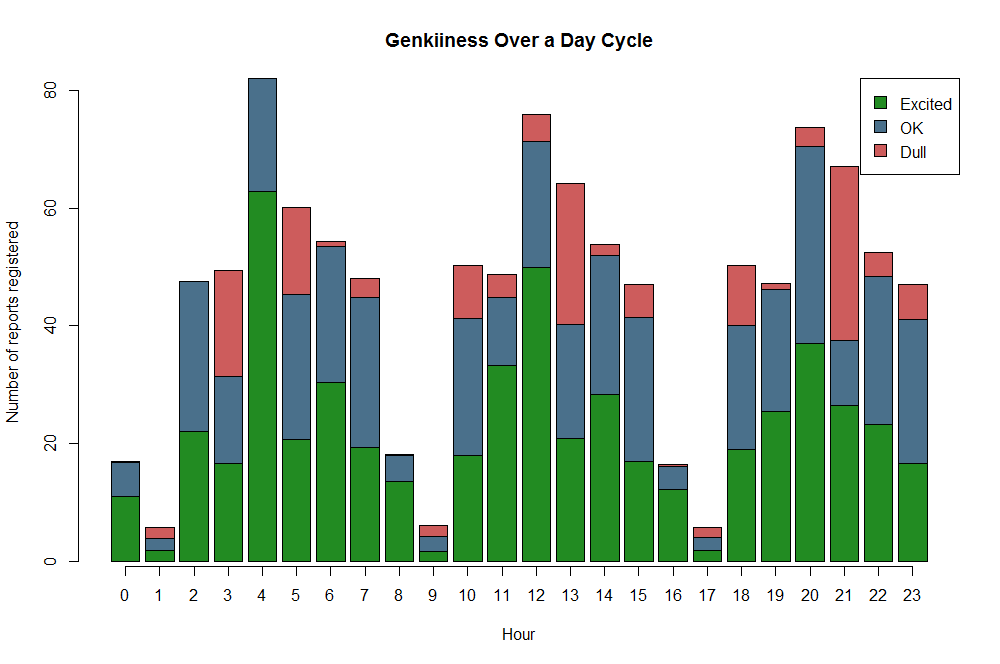
\includegraphics[width=1\linewidth]{images/GenkioverDay}
		\caption{Captured feelings over a day cycle.\label{fig:genkiioverday}}
	\end{center}
\end{figure}

The fact that we used a total of 1059 reports to construct this visualization seems to help us capture a overall stable group behavior. The daily activity is clearly separated in 8 hour periods.

In contrast the higher amount of reports seems to be made around 4, 12 and 20. Once again we can hypothesize that around 4 we have a lot of reports from people going out at night. The highest peak of our registered reports happens just before the public transport resumes in the city of Tokyo (around 5). Although the relative proportion of emotions reported seems not to vary much throughout the day, the 3, 4, and 5 seem to be privileged time for expressing emotions. In the 4 a.m. slot we captured the highest peak of ''Feeling Happy'' report. The 3 and 5 a.m. slots see some of the highest proportions of ''Feeling Sad'' reports.

Meal times or meal breaks seem also to be privileged by users to make reports. 
We always verify during the hour after the slot with a report peak there is a rise on general dissatisfaction, which is interesting because the peak report times (4,12, and 20) also represent peaks of the ''Feeling Happy'' reports.

These results reinforce that users tend to use the Genkii app as a pastime. 

\subsection{Gestures} 
The accuracy (the gesture predicted by the system being the same as the gesture confirmed), is 85.3\% for the first campaign, and 83.6\% for the second campaign.
The prevalence of left-handed people is similar in both campaigns with 7\% of self reported left-handed people in the first campaign, and 10\% on the second campaign. Overall the percentage of left-handed people was 9.7\%.

The confirmed accuracy of the gesture predicted was 85\% for the paid reports and 84.3\% for non-rewarded reports. Once again there seems not to be a significant difference between reports that are rewarded and non-rewarded reports.

\section{Discussion}

Despite the inherent advantages of time and reach cost, crowdsourced studies end up forgoing the control over the experimental setting. It is difficult to assure conditions for representative demographics. 
This fine grained control can be replaced by large numbers in statistical sampling. 


During the first campaign, using fixed rewards, we noticed that 19\% of the users that provide reports ended up providing more reports than the strictly rewarded ones.
This points us to the merit of the application in capturing the users' interest. 
Perhaps the effect of the stable reward experiment made users shift their focus from the reward acquisition to the application. Besides clearly displaying the instructions, and the presence of the timer, Genkii allows the user to explore and play with the application, making reports (as long as successive reports are not made in the same place).
 
The design decision to use gestures started as a way to promote a mechanical task but ended up providing a playful way to make a Genkii report, which made the non-rewarded reports around 35\% of all reports registered. This points to the fact that Genkii succeeds in keeping the users interested, and motivated without inducements. This brings us to an important conclusion: careful design, and toy/game like attributes play an important role in keeping the users engaged. We can go even further in stating that in general we did not verify a difference in the quality of reports, because the relative proportions remain practically the same whether the users unlock a reward or not.

From the data captured from the application we were able to categorize the population who enrolled to try the Genkii application and get rewarded by doing so. We found out that most people who joined have a certain degree of mobility, which we associated with commuting. It was also interesting to find that the usage of the application has a periodic behavior, with 8 hour cycles, and there seems to be two mood related changes during those cycles. During the peak reporting times, the ''Felling Happy'' mood proportion tens to increase slightly, while during the following our we experience an increase in ''Feeling Sad'' reports.  

In terms of Yahoo Crowdsourcing campaigns we learned that the first three to four days saw the highest number of new users. This may be a limitation in the way the tasks are  promoted in Yahoo Crowdsoucing Japan website, but may be helpful for future campaign design. 

The biggest bridge in terms of user droprate, as expected is between the first and the second report. Still, when considering user completed tasks, this  droprate was more accentuated when the initial reward was bigger.





 


\section{Conclusions}






Future developments for Genkii include the application of the knowledge acquired to new areas, such as pain monitoring, disaster response. In either case it would be to our advantage if the application was able to trigger intrinsic motivation in its users.
During the campaigns' time Genkii registered a significant percentage of unpaid reports (around 35\%).  

In this study, we considered only the usage of monetary inducements. There's an extensive literature on gamification, and the usage of other methods to keep the users engaged. Future steps include offering a version with gamification elements, and after a similar user acquisition compare the engagement and drop rates of the study.

The emotional report data collected seems to plausibly explain trends and cultural aspects. One future work could be trying to match and validate this emotional report method with sentiment analysis from Twitter, for example. 



\section{ Acknowledgments}

We thank Daniel Morais for his contribution on the visualization of the Genkii Map website.

%\section{Copyright}
%All papers submitted for publication by AAAI Press must be accompanied by a valid signed copyright form or, in the case of technical reports, by a valid signed permission to distribute form. There are no exceptions to this requirement. You must send us the original version of this form. However, to meet the deadline, you may fax (1-650-321-4457) or scan and e-mail the form (pubforms15@aaai.org) to AAAI by the submission deadline, and then mail the original via postal mail to the AAAI office. \textbf{If you fail to send in a signed copyright or permission form, your paper will not be published.} You will find PDF versions of the AAAI copyright and permission to distribute forms in the author kit.
%
%\section{Formatting Requirements in Brief}
%We need source and PDF files that can be used in a variety of ways and can be output on a variety of devices. AAAI imposes some requirements on your source and PDF files that must be followed. Most of these requirements are based on our efforts to standardize conference manuscript properties and layout. These requirements are as follows, and all papers submitted to AAAI for publication must comply:
%
%\begin{itemize}
%\item Your .tex file must compile in PDF\LaTeX{} --- \textbf{ no .ps or .eps figure files.}
%\item All fonts must be embedded in the PDF file --- \textbf{ this includes your figures.}
%\item Modifications to the style sheet (or your document) in an effort to avoid extra page charges are NOT allowed.
%\item No type 3 fonts may be used (even in illustrations).
%\item Your title must follow US capitalization rules.
%\item \LaTeX{} documents must use the Times or Nimbus font package (do not use Computer Modern for the text of your paper).
%\item No \LaTeX{} 209 documents may be used or submitted.
%\item Fonts that require non-English language support (CID and Identity-H) must be converted to outlines or removed from the document (even if they are in a graphics file embedded in the document). 
%\item Two-column format in AAAI style is required for all papers.
%\item The paper size for final submission must be US letter. No exceptions.
%\item The source file must exactly match the PDF.
%\item The document margins must be as specified in the formatting instructions.
%\item The number of pages and the file size must be as specified for your event.
%\item No document may be password protected.
%\item Neither the PDFs nor the source may contain any embedded links or bookmarks.
%\item Your source and PDF must not have any page numbers, footers, or headers.
%\item Your PDF must be compatible with Acrobat 5 or higher.
%\item Your \LaTeX{} source file (excluding references) must consist of a \textbf{single} file (use of the ``input" command is not allowed.
%\item Your graphics must be sized appropriately outside of \LaTeX{} (do not use the ``clip" command) .
%\end{itemize}
%
%If you do not follow the above requirements, it is likely that we will be unable to publish your paper.
%
%\section{What Files to Submit}
%You must submit the following items to ensure that your paper is published:
%\begin{itemize}
%\item A fully-compliant PDF file.
%\item Your  \LaTeX{}  source file submitted as a \textbf{single} .tex file (do not use the ``input" command to include sections of your paper --- every section must be in the single source file). The only exception is the bibliography, which you may include separately. Your source must compile on our system, which includes the standard \LaTeX{} support files.
%\item All your graphics files.
%\item The \LaTeX{}-generated files (e.g. .aux and .bib file, etc.) for your compiled source.
%\item All the nonstandard style files (ones not commonly found in standard \LaTeX{} installations) used in your document (including, for example, old algorithm style files). If in doubt, include it.
%\end{itemize}
%
%Your \LaTeX{} source will be reviewed and recompiled on our system (if it does not compile, you may incur late fees).   \textbf{Do not submit your source in multiple text files.} Your single \LaTeX{} source file must include all your text, your bibliography (formatted using aaai.bst), and any custom macros. Accompanying this source file, you must also supply any nonstandard (or older) referenced style files and all your referenced graphics files. 
%
%Your files should work without any supporting files (other than the program itself) on any computer with a standard \LaTeX{} distribution. Place your PDF and source files in a single tar, zipped, gzipped, stuffed, or compressed archive. Name your source file with your last (family) name.
%
%\textbf{Do not send files that are not actually used in the paper.} We don't want you to send us any files not needed for compiling your paper, including, for example, this instructions file, unused graphics files, and so forth.  A shell script (created by an AAAI member --- it might not work without modification on your system) that might help you create the \LaTeX{} source package is included in the Author Kit.
%
%\section{Using \LaTeX{} to Format Your Paper}
%
%The latest version of the AAAI style file is available on AAAI's website. Download this file and place it in a file named ``aaai.sty" in the \TeX\ search path. Placing it in the same directory as the paper should also work. You must download the latest version of the complete author kit so that you will have the latest instruction set.
%
%\subsection{Document Preamble}
%
%In the \LaTeX{} source for your paper, you \textbf{must} place the following lines as shown in the example in this subsection. This command set-up is for three authors. Add or subtract author and address lines as necessary, and uncomment the portions that apply to you. In most instances, this is all you need to do to format your paper in the Times font. The helvet package will cause Helvetica to be used for sans serif, and the courier package will cause Courier to be used for the typewriter font. These files are part of the PSNFSS2e package, which is freely available from many Internet sites (and is often part of a standard installation).
%
%Leave the setcounter for section number depth commented out and set at 0 unless you want to add section numbers to your paper. If you do add section numbers, you must uncomment this line and change the number to 1 (for section numbers), or 2 (for section and subsection numbers). The style file will not work properly with numbering of subsubsections, so do not use a number higher than 2.
%
%
%\begin{quote}
%\begin{small}
%\textbackslash documentclass[letterpaper]{article}\\
%\% \textit{Required Packages}\\
%\textbackslash usepackage\{aaai\}\\
%\textbackslash usepackage\{times\}\\
%\textbackslash usepackage\{helvet\}\\
%\textbackslash usepackage\{courier\}\\
%\textbackslash setlength\{\textbackslash pdfpagewidth\}\{8.5in\}
%\textbackslash setlength\{\textbackslash pdfpageheight\}\{11in\}\\
%\%\%\%\%\%\%\%\%\%\%\\
%\% \textit{PDFINFO for PDF\LaTeX{}}\\
%\% Uncomment and complete the following for metadata (your paper must compile with PDF\LaTeX{})\\
%\textbackslash pdfinfo\{\\
%/Title (Input Your Paper Title Here)\\
%/Author (John Doe, Jane Doe)\\
%/Keywords (Input your paper's keywords in this optional area)\\
%\}\\
%\%\%\%\%\%\%\%\%\%\%\\
%\% \textit{Section Numbers}\\
%\% Uncomment if you want to use section numbers\\
%\% and change the 0 to a 1 or 2\\
%\% \textbackslash setcounter\{secnumdepth\}\{0\}\\
%\%\%\%\%\%\%\%\%\%\%\\
%\% \textit{Title, Author, and Address Information}\\
%\textbackslash title\{Title\}\\
%\textbackslash author\{Author 1 \textbackslash and Author 2\textbackslash\textbackslash \\ 
%Address line\textbackslash\textbackslash\\ Address line\textbackslash\textbackslash \\
%\textbackslash And\\
%Author 3\textbackslash\textbackslash\\ Address line\textbackslash\textbackslash\\ Address line\}\\
%\%\%\%\%\%\%\%\%\%\%\\
%\% \textit{Body of Paper Begins}\\
%\textbackslash begin\{document\}\\
%\textbackslash maketitle\\
%...\\
%\%\%\%\%\%\%\%\%\%\%\\
%\% \textit{References and End of Paper}\\
%\textbackslash bibliography\{Bibliography-File\}\\
%\textbackslash bibliographystyle\{aaai\}\\
%\textbackslash end\{document\}
%\end{small}
%\end{quote}
%
%\subsection{Inserting Document Metadata with \LaTeX{}}
%PDF files contain document summary information that enables us to create an Acrobat index (pdx) file, and also allows search engines to locate and present your paper more accurately. \textbf{Document Metadata  for Author and Title are REQUIRED.} 
%
%If your paper includes illustrations that are not compatible with PDF\TeX{} (such as .eps or .ps documents), you will need to convert them. The epstopdf package will usually work for eps files. You will need to convert your ps files to PDF however.
%
%\textit{Important:} Do not include \textit{any} \LaTeX{} code or nonascii characters (including accented characters) in the metadata. The data in the metadata must be completely plain ascii. It may not include slashes, accents, linebreaks, unicode, or any \LaTeX{} commands. Type the title exactly as it appears on the paper (minus all formatting). Input the author names in the order in which they appear on the paper (minus all accents), separating each author by a comma. You may also include keywords in the Keywords field.
%
%
%
%\subsection{Preparing Your Paper}
%
%After the preamble above, you should prepare your paper as follows:
%
%\begin{quote}
%\begin{small}
%\textbackslash begin\{document\}\\
%\textbackslash maketitle\\
%...\\
%\textbackslash bibliography\{Bibliography-File\}\\
%\textbackslash bibliographystyle\{aaai\}\\
%\textbackslash end\{document\}\\
%\end{small}
%\end{quote}
%\subsection{Incompatible Packages}
%The following packages are incompatible with aaai.sty and/or aaai.bst and must not be used (this list is not exhaustive --- there are others as well):
%\begin{itemize}
%\item hyperref
%\item natbib
%\item geometry
%\item titlesec
%\item layout
%\item caption
%\item titlesec
%\item savetrees
%\item T1 fontenc package (install the CM super fonts package instead)
%\end{itemize}
%
%\subsection{Illegal Commands}
%The following commands may not be used in your paper:
%\begin{itemize}
%\item \textbackslash input
%\item \textbackslash vspace (when used before or after a section or subsection)
%\item \textbackslash addtolength 
%\item \textbackslash columnsep
%\item \textbackslash top margin (or text height or addsidemargin or even side margin)
%\item trim or clip (used to crop figures)
%\end{itemize}
%
%\subsection{Paper Size, Margins, and Column Width}
%Papers must be formatted to print in two-column format on 8.5 x 11 inch US letter-sized paper. The margins must be exactly as follows: 
%\begin{itemize}
%\item Top margin: .75 inches
%\item Left margin: .75 inches
%\item Right margin: .75 inches
%\item Bottom margin: 1.25 inches
%\end{itemize} 
%
%
%The default paper size in most installations of \LaTeX{} is A4. However, because we require that your electronic paper be formatted in US letter size, you will need to alter the default for this paper to US letter size. Assuming you are using the 2e version of \LaTeX{}, you can do this by including the [letterpaper] option at the beginning of your file: 
%\textbackslash documentclass[letterpaper]{article}. 
%
%This command is usually sufficient to change the format. Sometimes, however, it may not work. Use PDF\LaTeX{} and include
%\textbackslash setlength\{\textbackslash pdfpagewidth\}\{8.5in\}
%\textbackslash setlength\{\textbackslash pdfpageheight\}\{11in\}
%in your preamble. 
%
%\textbf{Do not use the Geometry package to alter the page size.} Use of this style file alters aaai.sty and will result in your paper being rejected. 
%
%
%\subsubsection{Column Width and Margins.}
%To ensure maximum readability, your paper must include two columns. Each column should be 3.3 inches wide (slightly more than 3.25 inches), with a .375 inch (.952 cm) gutter of white space between the two columns. The aaai.sty file will automatically create these columns for you. 
%
%\subsection{Overlength Papers}
%If your paper is too long, turn on \textbackslash frenchspacing, which will reduce the space after periods. Next,  shrink the size of your graphics. Use \textbackslash centering instead of \textbackslash begin\{center\} in your figure environment. If these two methods don't work, you may minimally use the following. For floats (tables and figures), you may minimally reduce \textbackslash floatsep, \textbackslash textfloatsep, \textbackslash abovecaptionskip, and \textbackslash belowcaptionskip. For mathematical environments, you may minimally reduce \textbackslash abovedisplayskip, \textbackslash belowdisplayskip, and \textbackslash arraycolsep. You may also alter the size of your bibliography by inserting \textbackslash fontsize\{9.5pt\}\{10.5pt\} \textbackslash selectfont
%right before the bibliography. 
%
%Commands that alter page layout are forbidden. These include \textbackslash columnsep, \textbackslash topmargin, \textbackslash topskip, \textbackslash textheight, \textbackslash textwidth, \textbackslash oddsidemargin, and \textbackslash evensizemargin (this list is not exhaustive). If you alter page layout, you will be required to pay the page fee \textit{plus} a reformatting fee. Other commands that are questionable and may cause your paper to be rejected include  \textbackslash parindent, and \textbackslash parskip. Commands that alter the space between sections are also questionable. The title sec package is not allowed. Regardless of the above, if your paper is obviously ``squeezed" it is not going to to be accepted. Before using every trick you know to make your paper a certain length, try reducing the size of your graphics or cutting text instead or (if allowed) paying the extra page charge. It will be cheaper in the long run.
%
%\subsection{Figures}
%Your paper must compile in PDF\LaTeX{}. Consequently, all your figures must be .jpg, .png, or .pdf. You may not use the .gif (the resolution is too low), .ps, or .eps file format for your figures.
%
%When you include your figures, you must crop them \textbf{outside} of \LaTeX{}. The command \textbackslash includegraphics*[clip=true, viewport 0 0 10 10]{...} might result in a PDF that looks great, but the image is \textbf{not really cropped.} The full image can reappear when page numbers are applied or color space is standardized. 
%
%\subsection{Type Font and Size}
%Your paper must be formatted in Times Roman or Nimbus. We will not accept papers formatted using Computer Modern or Palatino or some other font as the text or heading typeface. Sans serif, when used, should be Courier. Use Symbol or Lucida or Computer Modern for \textit{mathematics only. } 
%
%Do not use type 3 fonts for any portion of your paper, including graphics. Type 3 bitmapped fonts are designed for fixed resolution printers. Most print at 300 dpi even if the printer resolution is 1200 dpi or higher. They also often cause high resolution imagesetter devices and our PDF indexing software to crash. Consequently, AAAI will not accept electronic files containing obsolete type 3 fonts. Files containing those fonts (even in graphics) will be rejected. 
%
%Fortunately, there are effective workarounds that will prevent your file from embedding type 3 bitmapped fonts. The easiest workaround is to use the required times, helvet, and courier packages with \LaTeX{}2e. (Note that papers formatted in this way will still use Computer Modern for the mathematics. To make the math look good, you'll either have to use Symbol or Lucida, or you will need to install type 1 Computer Modern fonts --- for more on these fonts, see the section ``Obtaining Type 1 Computer Modern.")
%
%If you are unsure if your paper contains type 3 fonts, view the PDF in Acrobat Reader. The Properties/Fonts window will display the font name, font type, and encoding properties of all the fonts in the document. If you are unsure if your graphics contain type 3 fonts (and they are PostScript or encapsulated PostScript documents), create PDF versions of them, and consult the properties window in Acrobat Reader. 
%
%The default size for your type should be ten-point with twelve-point leading (line spacing). Start all pages (except the first) directly under the top margin. (See the next section for instructions on formatting the title page.) Indent ten points when beginning a new paragraph, unless the paragraph begins directly below a heading or subheading.
%
%\subsubsection{Obtaining Type 1 Computer Modern for \LaTeX{}.}
%
%If you use Computer Modern for the mathematics in your paper (you cannot use it for the text) you may need to download type 1 Computer fonts. They are available without charge from the American Mathematical Society:
%http://www.ams.org/tex/type1-fonts.html. 
%
%\subsection{Title and Authors}
%Your title must appear in mixed case (nouns, pronouns, and verbs are capitalized) near the top of the first page, centered over both columns in sixteen-point bold type (twenty-four point leading). This style is called ``mixed case." Author's names should appear below the title of the paper, centered in twelve-point type (with fifteen point leading), along with affiliation(s) and complete address(es) (including electronic mail address if available) in nine-point roman type (the twelve point leading). (If the title is long, or you have many authors, you may reduce the specified point sizes by up to two points.) You should begin the two-column format when you come to the abstract. 
%
%\subsubsection{Formatting Author Information}
%Author information can be set in a number of different styles, depending on the number of authors and the number of affiliations you need to display. For several authors from the same institution, use \textbackslash and:
%
%\begin{quote}
%\begin{small}
%\textbackslash author\{Author 1 \textbackslash and  ...  \textbackslash and Author \textit{n}\textbackslash \textbackslash  \\
%Address line \textbackslash \textbackslash ~... \textbackslash \textbackslash ~Address line\}
%\end{small}
%\end{quote}
%
%\noindent If the names do not fit well on one line use:
%
%\begin{quote}
%\begin{small}
%\textbackslash author\{Author 1\}\textbackslash \textbackslash \\ \{\textbackslash bf Author 2\}\textbackslash \textbackslash ~ 
%... \textbackslash \textbackslash ~\{\textbackslash bf Author \textit{n}\}\textbackslash \textbackslash \\
%Address line \textbackslash \textbackslash ~ ... \textbackslash \textbackslash ~ Address line\}
%\end{small}
%\end{quote}
%
%\noindent For authors from different institutions, use \textbackslash And:
%
%\begin{quote}
%\begin{small}
%\textbackslash author\{Author 1\textbackslash \textbackslash ~ Address line \textbackslash \textbackslash ~...  \textbackslash \textbackslash ~ Address line
%\textbackslash And  ...  
%\textbackslash And
%Author \textit{n}\textbackslash \textbackslash \\ Address line\textbackslash \textbackslash ~
%... \textbackslash \textbackslash ~
%Address line\}
%\end{small}
%\end{quote}
%
%\noindent To start a separate ``row" of authors, use \textbackslash AND:
%\begin{quote}
%\begin{small}
%\textbackslash author\{Author 1\textbackslash\textbackslash ~ Address line \textbackslash\textbackslash ~
%...  \textbackslash \textbackslash ~ Address line\textbackslash\textbackslash \\
%\textbackslash AND\\
%Author 2 \textbackslash\textbackslash ~ Address line \textbackslash\textbackslash ~
%...  \textbackslash \textbackslash ~ Address line\textbackslash\textbackslash \\
%\textbackslash And\\
%Author 3 \textbackslash\textbackslash ~ Address line \textbackslash\textbackslash ~
%...  \textbackslash \textbackslash ~ Address line\textbackslash\textbackslash \\\}
%\end{small}
%\end{quote}
%
%\noindent If the title and author information does not fit in the area allocated, place
%\textbackslash setlength\textbackslash titlebox\{\textit{height}\}
%after the \textbackslash documentclass line where \{\textit{height}\} is something like 2.5in.
%
%\subsection{\LaTeX{} Copyright Notice}
%The copyright notice automatically appears if you use aaai.sty. If you are creating a technical report, it is not necessary to include this notice. You may disable the copyright line using the \verb+\+nocopyrightcommand. To change the entire text of the copyright slug, use:
%\textbackslash copyrighttext \{\emph{text}\}.
%Either of these must appear before \textbackslash maketitle. Please be advised, however, that \textit{if you disable or change the copyright line and transfer of copyright is required, your paper will not be published.}
%
%\subsection{Credits}
%Any credits to a sponsoring agency should appear in the acknowledgments section, unless the agency requires different placement. If it is necessary to include this information on the front page, use
%\textbackslash thanks in either the \textbackslash author or \textbackslash title commands.
%For example:
%\begin{quote}
%\begin{small}
%\textbackslash title\{Very Important Results in AI\textbackslash thanks\{This work is
% supported by everybody.\}\}
%\end{small}
%\end{quote}
%Multiple \textbackslash thanks commands can be given. Each will result in a separate footnote indication in the author or title with the corresponding text at the botton of the first column of the document. Note that the \textbackslash thanks command is fragile. You will need to use \textbackslash protect.
%
%Please do not include \textbackslash pubnote commands in your document.
%
%\subsection{Abstract}
%The abstract must be placed at the beginning of the first column, indented ten points from the left and right margins. The title �Abstract� should appear in ten-point bold type, centered above the body of the abstract. The abstract should be set in nine-point type with ten-point leading. This concise, one-paragraph summary should describe the general thesis and conclusion of your paper. A reader should be able to learn the purpose of the paper and the reason for its importance from the abstract. The abstract should be no more than two hundred words in length. (Authors who are submitting short one- or two-page extended extracts should provide a short abstract of only a sentence or so.) \textbf{Do not include references in your abstract!}
%
%\subsection{Page Numbers}
%
%Do not \textbf{ever} print any page numbers on your paper. 
%
%\subsection{Text }
%The main body of the paper must be formatted in ten-point with twelve-point leading (line spacing).
%
%\subsection{Citations}
%Citations within the text should include the author's last name and year, for example (Newell 1980). Append lower-case letters to the year in cases of ambiguity. Multiple authors should be treated as follows: (Feigenbaum and Engelmore 1988) or (Ford, Hayes, and Glymour 1992). In the case of four or more authors, list only the first author, followed by et al. (Ford et al. 1997).
%
%\subsection{Extracts}
%Long quotations and extracts should be indented ten points from the left and right margins. 
%
%\begin{quote}
%This is an example of an extract or quotation. Note the indent on both sides. Quotation marks are not necessary if you offset the text in a block like this, and properly identify and cite the quotation in the text. 
%
%\end{quote}
%
%\subsection{Footnotes}
%Avoid footnotes as much as possible; they interrupt the reading of the text. When essential, they should be consecutively numbered throughout with superscript Arabic numbers. Footnotes should appear at the bottom of the page, separated from the text by a blank line space and a thin, half-point rule. 
%
%\subsection{Headings and Sections}
%When necessary, headings should be used to separate major sections of your paper. Remember, you are writing a short paper, not a lengthy book! An overabundance of headings will tend to make your paper look more like an outline than a paper.
%
%First-level heads should be twelve-point Times Roman bold type, mixed case (initial capitals followed by lower case on all words except articles, conjunctions, and prepositions, which should appear entirely in lower case), with fifteen-point leading, centered, with one blank line preceding them and three additional points of leading following them. Second-level headings should be eleven-point Times Roman bold type, mixed case, with thirteen-point leading, flush left, with one blank line preceding them and three additional points of leading following them. Do not skip a line between paragraphs. Third-level headings should be run in with the text, ten-point Times Roman bold type, mixed case, with twelve-point leading, flush left, with six points of additional space preceding them and no additional points of leading following them.
%
%\subsubsection{Section Numbers}
%The use of section numbers in AAAI Press papers is optional. To use section numbers in \LaTeX{}, uncomment the setcounter line in your document preamble and change the 0 to a 1 or 2. Section numbers should not be used in short poster papers.
%
%\subsubsection{Section Headings.}
%Sections should be arranged and headed as follows: 
%
%\subsubsection{Acknowledgments.}
%The acknowledgments section, if included, appears after the main body of text and is headed ``Acknowledgments." This section includes acknowledgments of help from associates and colleagues, credits to sponsoring agencies, financial support, and permission to publish. Please acknowledge other contributors, grant support, and so forth, in this section. Do not put acknowledgments in a footnote on the first page. If your grant agency requires acknowledgment of the grant on page 1, limit the footnote to the required statement, and put the remaining acknowledgments at the back. Please try to limit acknowledgments to no more than three sentences. 
%
%\subsubsection{Appendices.}
%Any appendices follow the acknowledgments, if included, or after the main body of text if no acknowledgments appear. 
%
%\subsubsection{References}
%The references section should be labeled ``References" and should appear at the very end of the paper (don't end the paper with references, and then put a figure by itself on the last page). A sample list of references is given later on in these instructions. Please use a consistent format for references. Poorly prepared or sloppy references reflect badly on the quality of your paper and your research. Please prepare complete and accurate citations. \cite{Choi2014}
%
%\subsection{Illustrations and Figures}
%Figures, drawings, tables, and photographs should be placed throughout the paper near the place where they are first discussed. Do not group them together at the end of the paper. If placed at the top or bottom of the paper, illustrations may run across both columns. Figures must not invade the top, bottom, or side margin areas. Figures must be inserted using the \textbackslash usepackage\{graphicx\}. Number figures sequentially, for example, figure 1, and so on. 
%
%The illustration number and caption should appear under the illustration. Labels, and other text in illustrations must be at least nine-point type. 
%
%\subsubsection{Low-Resolution Bitmaps.}
%You may not use low-resolution (such as 72 dpi) screen-dumps and GIF files---these files contain so few pixels that they are always blurry, and illegible when printed. If they are color, they will become an indecipherable mess when converted to black and white. This is always the case with gif files, which should never be used. The resolution of screen dumps can be increased by reducing the print size of the original file while retaining the same number of pixels. You can also enlarge files by manipulating them in software such as PhotoShop. Your figures should be a minimum of 266 dpi when incorporated into your document.
%
%\subsubsection{\LaTeX{} Overflow.}
%\LaTeX{} users please beware: \LaTeX{} will sometimes put portions of the figure or table or an equation in the margin. If this happens, you need to scale the figure or table down, or reformat the equation. Check your log file! You must fix any overflow into the margin (that means no overfull boxes in \LaTeX{}). If you don't, the overflow text will simply be eliminated. \textbf{Nothing is permitted to intrude into the margins.}
%
%\subsubsection{Using Color.}
%Your paper will be printed in black and white and grayscale. Consequently, because conversion to grayscale can cause undesirable effects (red changes to black, yellow can disappear, and so forth), we strongly suggest you avoid placing color figures in your document. Of course, any reference to color will be indecipherable to your reader. 
%
%\subsubsection{Drawings.}
%We suggest you use computer drawing software (such as Adobe Illustrator or, (if unavoidable), the drawing tools in Microsoft Word) to create your illustrations. Do not use Microsoft Publisher. These illustrations will look best if all line widths are uniform (half- to two-point in size), and you do not create labels over shaded areas. Shading should be 133 lines per inch if possible. Use Times Roman or Helvetica for all figure call-outs. \textbf{Do not use hairline width lines} --- be sure that the stroke width of all lines is at least .5 pt. Zero point lines will print on a laser printer, but will completely disappear on the high-resolution devices used by our printers.
%
%\subsubsection{Photographs and Images.}
%Photographs and other images should be in grayscale (color photographs will not reproduce well; for example, red tones will reproduce as black, yellow may turn to white, and so forth) and set to a minimum of 266 dpi. Do not prescreen images.
%
%\subsubsection{Resizing Graphics.}
%Resize your graphics \textbf{before} you include them with LaTeX. You may \textbf{not} use trim or clip options as part of your \textbackslash includgraphics command. Resize the media box of your PDF using a graphics program instead. 
%
%\subsubsection{Fonts in Your Illustrations}
%You must embed all fonts in your graphics before including them in your LaTeX document.
%
%\subsection{References} 
%
%
%
%
%The aaai.sty file includes a set of definitions for use in formatting references with BibTeX. These definitions make the bibliography style fairly close to the one specified below. To use these definitions, you also need the BibTeX style file ``aaai.bst," available in the author kit on the AAAI web site. Then, at the end of your paper but before \textbackslash end{document}, you need to put the following lines:
%
%\begin{quote}
%\begin{small}
%\textbackslash bibliographystyle\{aaai\}
%\textbackslash bibliography\{bibfile1,bibfile2,...\}
%\end{small}
%\end{quote}
%
%The list of files in the \textbackslash  bibliography command should be the names of your BibTeX source files (that is, the .bib files referenced in your paper).
%
%The following commands are available for your use in citing references:
%\begin{quote}
%\begin{small}
%\textbackslash cite: Cites the given reference(s) with a full citation. This appears as ``(Author Year)'' for one reference, or ``(Author Year; Author Year)'' for multiple references.\\
%\textbackslash shortcite: Cites the given reference(s) with just the year. This appears as ``(Year)'' for one reference, or ``(Year; Year)'' for multiple references.\\
%\textbackslash citeauthor: Cites the given reference(s) with just the author name(s) and no parentheses.\\
%\textbackslash citeyear: Cites the given reference(s) with just the date(s) and no parentheses.
%\end{small}
%\end{quote}
%
%\textbf{Warning:} The aaai.sty file is incompatible with the hyperref and natbib packages. If you use either, your references will be garbled and your paper will not be published.
%
%Formatted bibliographies should look like the following examples.
%
%\smallskip \noindent \textit{Book with Multiple Authors}\\
%Engelmore, R., and Morgan, A. eds. 1986. \textit{Blackboard Systems.} Reading, Mass.: Addison-Wesley.
%
%\smallskip \noindent \textit{Journal Article}\\
%Robinson, A. L. 1980a. New Ways to Make Microcircuits Smaller. \textit{Science} 208: 1019--1026.
%
%\smallskip \noindent \textit{Magazine Article}\\
%Hasling, D. W.; Clancey, W. J.; and Rennels, G. R. 1983. Strategic Explanations in Consultation. \textit{The International Journal of Man-Machine Studies} 20(1): 3--19.
%
%\smallskip \noindent \textit{Proceedings Paper Published by a Society}\\
%Clancey, W. J. 1983b. Communication, Simulation, and Intelligent Agents: Implications of Personal Intelligent Machines for Medical Education. In Proceedings of the Eighth International Joint Conference on Artificial Intelligence, 556--560. Menlo Park, Calif.: International Joint Conferences on Artificial Intelligence, Inc.
%
%\smallskip \noindent \textit{Proceedings Paper Published by a Press or Publisher}\\
%Clancey, W. J. 1984. Classification Problem Solving. In \textit{Proceedings of the Fourth National Conference on Artificial Intelligence,} 49--54. Menlo Park, Calif.: AAAI Press. 
%
%\smallskip \noindent \textit{University Technical Report}\\
%Rice, J. 1986. Poligon: A System for Parallel Problem Solving, Technical Report, KSL-86-19, Dept. of Computer Science, Stanford Univ. 
%
%\smallskip \noindent \textit{Dissertation or Thesis}\\
%Clancey, W. J. 1979b. Transfer of Rule-Based Expertise through a Tutorial Dialogue. Ph.D. diss., Dept. of Computer Science, Stanford Univ., Stanford, Calif.
%
%\smallskip \noindent \textit{Forthcoming Publication}\\
%Clancey, W. J. 1986a. The Engineering of Qualitative Models. Forthcoming.
%
%
%
%\section{Producing Reliable PDF\\Documents with \LaTeX{}}
%Generally speaking, PDF files are platform independent and accessible to everyone. When creating a paper for a proceedings or publication in which many PDF documents must be merged and then printed on high-resolution PostScript RIPs, several requirements must be met that are not normally of concern. Thus to ensure that your paper will look like it does when printed on your own machine, you must take several precautions:
%\begin{itemize}
%\item Use type 1 fonts (not type 3 fonts)
%\item Use only standard Times, Nimbus, and CMR font packages (not fonts like F3 or fonts with tildes in the names or fonts---other than Computer Modern---that are created for specific point sizes, like Times\~{}19) or fonts with strange combinations of numbers and letters
%\item Embed all fonts when producing the PDF
%\item Do not use the [T1]{fontenc} package (install the CM super fonts package instead)
%\end{itemize}
%
%\subsection{Creating Output Using PDF\LaTeX{} Is Required}
%By using the PDF\TeX{} program instead of straight \LaTeX{} or \TeX{}, you will probably avoid the type 3 font problem altogether (unless you use a package that calls for metafont). PDF\LaTeX{} enables you to create a PDF document directly from \LaTeX{} source. The one requirement of this software is that all your graphics and images must be available in a format that PDF\LaTeX{} understands (normally PDF).
%
%PDF\LaTeX{}'s default is to create documents with type 1 fonts. If you find that it is not doing so in your case, it is likely that one or more fonts are missing from your system or are not in a path that is known to PDF\LaTeX{}.
%
%\subsubsection{dvipdf Script}
%Scripts such as dvipdf which ostensibly bypass the Postscript intermediary should not be used since they generally do not instruct dvips to use the config.pdf file.
%
%\subsubsection{dvipdfm}
%Do not use this dvi-PDF conversion package if your document contains graphics (and we recommend you avoid it even if your document does not contain graphics).
%
%\subsection{Ghostscript}
%\LaTeX{} users should not use GhostScript to create their PDFs.
%
%\subsection{Graphics}
%If you are still finding type 3 fonts in your PDF file, look at your graphics! \LaTeX{} users should check all their imported graphics files as well for font problems.
%
%\section{Proofreading Your PDF}
%Please check all the pages of your PDF file. Is the page size A4? Are there any type 3, Identity-H, or CID fonts? Are all the fonts embedded? Are there any areas where equations or figures run into the margins? Did you include all your figures? Did you follow mixed case capitalization rules for your title? Did you include a copyright notice? Do any of the pages scroll slowly (because the graphics draw slowly on the page)? Are URLs underlined and in color? You will need to fix these common errors before submitting your file. 
%
%\section{Improperly Formatted Files }
%In the past, AAAI has corrected improperly formatted files submitted by the authors. Unfortunately, this has become an increasingly burdensome expense that we can no longer absorb. Consequently, if your file is improperly formatted, it may not be possible to include your paper in the publication. If time allows, however, you will be notified via e-mail (with a copy to the program chair) of the problems with your file and given the option of correcting the file yourself (and paying a late fee) or asking that AAAI have the file corrected for you, for an additional fee. If you opt to correct the file yourself, please note that we cannot provide you with any additional advice beyond that given in your packet. Files that are not corrected after a second attempt will be withdrawn.
%
%\subsection{\LaTeX{} 209 Warning}
%If you use \LaTeX{} 209 we will not be able to publish your paper. Convert your paper to \LaTeX{}2e.
%
%\section{Naming Your Electronic File}
%We request that you name your \LaTeX{} source file with your last name (family name) so that it can easily be differentiated from other submissions. If you name your files with the name of the event or ``aaai" or ``paper" or ``camera-ready" or some other generic or indecipherable name, you bear all risks of loss --- it is extremely likely that your file may be overwritten.
%
%\section{Submitting Your Electronic Files to AAAI}
%Submitting your files to AAAI is a two-step process. It is explained fully in the author registration and submission instructions. Please consult this document for details on how to submit your paper.
%
%\section{Inquiries} 
%If you have any questions about the preparation or submission of your paper as instructed in this document, please contact AAAI Press at the address given below. If you have technical questions about implementation of the aaai style file, please contact an expert at your site. We do not provide technical support for \LaTeX{} or any other software package. To avoid problems, please keep your paper simple, and do not incorporate complicated macros and style files.
%
%\begin{quote}
%\noindent AAAI Press\\
%2275 East Bayshore Road, Suite 160\\
%Palo Alto, California 94303\\ 
%\textit{Telephone:} (650) 328-3123\\ 
%\textit{E-mail:} See the submission instructions for your particular conference or event.
%\end{quote}
%
%\section{Additional Resources}
%\LaTeX{} is a difficult program to master. If you've used that software, and this document didn't help or some items were not explained clearly, we recommend you read Michael Shell's excellent document (testflow doc.txt V1.0a 2002/08/13) about obtaining correct PS/PDF output on \LaTeX{} systems. (It was written for another purpose, but it has general application as well). It is available at www.ctan.org in the tex-archive.
%
%\section{ Acknowledgments}
%AAAI is especially grateful to Peter Patel Schneider for his work in implementing the aaai.sty file, liberally using the ideas of other style hackers, including Barbara Beeton. We also acknowledge with thanks the work of George Ferguson for his guide to using the style and BibTeX files --- which has been incorporated into this document  --- and Hans Guesgen, who provided several timely modifications, as well as the many others who have, from time to time, sent in suggestions on improvements to the AAAI style. 
%
%The preparation of the \LaTeX{} and Bib\TeX{} files that implement these instructions was supported by Schlumberger Palo Alto Research, AT\&T Bell Laboratories, Morgan Kaufmann Publishers, The Live Oak Press, LLC, and AAAI Press. Bibliography style changes were added by Sunil Issar. \verb+\+pubnote was added by J. Scott Penberthy. George Ferguson added support for printing the AAAI copyright slug. Additional changes to aaai.sty and aaai.bst have been made by the AAAI staff.
%
%\bigskip
%\noindent Thank you for reading these instructions carefully. We look forward to receiving your electronic files!

\bibliographystyle{aaai}
\bibliography{genkiarticle}
\end{document}
